\documentclass{standalone}
\usepackage{tikz}
\usetikzlibrary{patterns, positioning}


\begin{document}
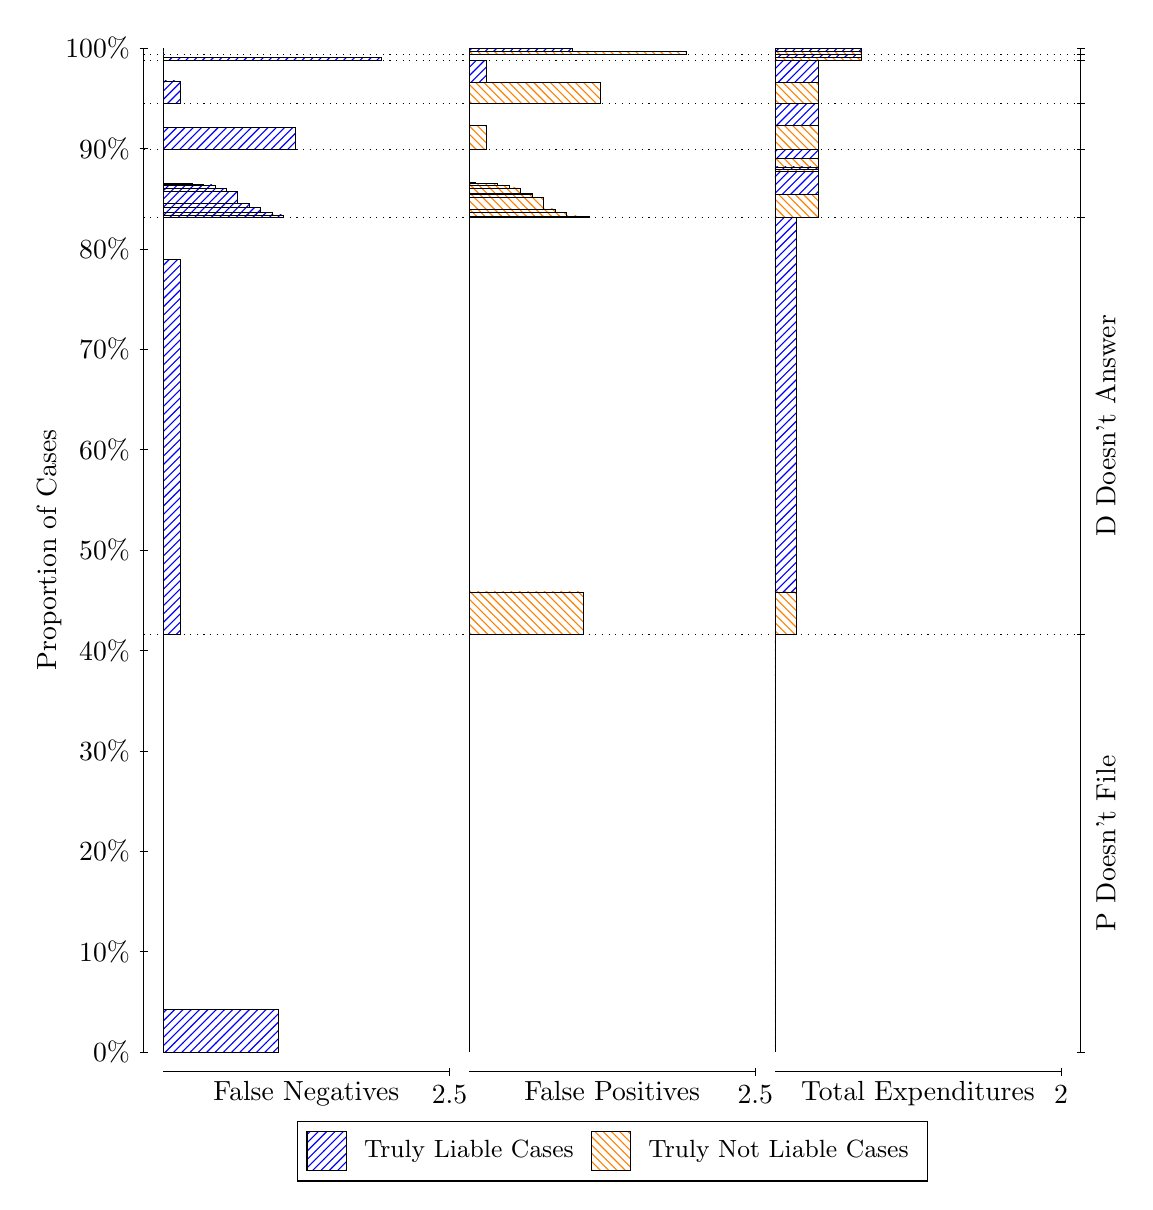
\begin{tikzpicture}
\draw[black, very thin] (1.5,1.75) -- (1.5,14.5);
\node[rotate=90, text=black, anchor=center] at (0.3, 8.125) {Proportion of Cases};
\draw[black, very thin] (1.45,1.75) -- (1.55,1.75);
\node[text=black, anchor=east] at (1.45, 1.75) {0\%};
\draw[black, very thin] (1.45,3.025) -- (1.55,3.025);
\node[text=black, anchor=east] at (1.45, 3.025) {10\%};
\draw[black, very thin] (1.45,4.3) -- (1.55,4.3);
\node[text=black, anchor=east] at (1.45, 4.3) {20\%};
\draw[black, very thin] (1.45,5.575) -- (1.55,5.575);
\node[text=black, anchor=east] at (1.45, 5.575) {30\%};
\draw[black, very thin] (1.45,6.85) -- (1.55,6.85);
\node[text=black, anchor=east] at (1.45, 6.85) {40\%};
\draw[black, very thin] (1.45,8.125) -- (1.55,8.125);
\node[text=black, anchor=east] at (1.45, 8.125) {50\%};
\draw[black, very thin] (1.45,9.4) -- (1.55,9.4);
\node[text=black, anchor=east] at (1.45, 9.4) {60\%};
\draw[black, very thin] (1.45,10.675) -- (1.55,10.675);
\node[text=black, anchor=east] at (1.45, 10.675) {70\%};
\draw[black, very thin] (1.45,11.95) -- (1.55,11.95);
\node[text=black, anchor=east] at (1.45, 11.95) {80\%};
\draw[black, very thin] (1.45,13.225) -- (1.55,13.225);
\node[text=black, anchor=east] at (1.45, 13.225) {90\%};
\draw[black, very thin] (1.45,14.5) -- (1.55,14.5);
\node[text=black, anchor=east] at (1.45, 14.5) {100\%};

\draw[black, very thin] (13.4,1.75) -- (13.4,14.5);
\draw[black, very thin] (13.35,1.75) -- (13.45,1.75);
\node[anchor=west] at (13.35, 1.75) {};
\draw[black, very thin] (13.35,7.0516) -- (13.45,7.0516);
\node[anchor=west] at (13.35, 7.0516) {};
\draw[black, very thin] (13.35,12.352) -- (13.45,12.352);
\node[anchor=west] at (13.35, 12.352) {};
\draw[black, very thin] (13.35,13.213) -- (13.45,13.213);
\node[anchor=west] at (13.35, 13.213) {};
\draw[black, very thin] (13.35,13.801) -- (13.45,13.801);
\node[anchor=west] at (13.35, 13.801) {};
\draw[black, very thin] (13.35,14.342) -- (13.45,14.342);
\node[anchor=west] at (13.35, 14.342) {};
\draw[black, very thin] (13.35,14.42) -- (13.45,14.42);
\node[anchor=west] at (13.35, 14.42) {};
\draw[black, very thin] (13.35,14.5) -- (13.45,14.5);
\node[anchor=west] at (13.35, 14.5) {};

\draw[black, very thin, pattern color=blue, pattern=north east lines] (1.75,1.75) rectangle (3.2033,2.2912);
\draw[black, very thin, pattern color=orange, pattern=north west lines] (1.75,2.2912) rectangle (1.75,7.0516);
\draw[black, very thin, pattern color=blue, pattern=north east lines] (1.75,7.0516) rectangle (1.968,11.811);
\draw[black, very thin, pattern color=orange, pattern=north west lines] (1.75,11.811) rectangle (1.75,12.352);
\draw[black, very thin, pattern color=blue, pattern=north east lines] (1.75,12.352) rectangle (3.276,12.38);
\draw[black, very thin, pattern color=blue, pattern=north east lines] (1.75,12.38) rectangle (3.1307,12.409);
\draw[black, very thin, pattern color=blue, pattern=north east lines] (1.75,12.409) rectangle (2.9853,12.478);
\draw[black, very thin, pattern color=blue, pattern=north east lines] (1.75,12.478) rectangle (2.84,12.53);
\draw[black, very thin, pattern color=blue, pattern=north east lines] (1.75,12.53) rectangle (2.6947,12.676);
\draw[black, very thin, pattern color=blue, pattern=north east lines] (1.75,12.676) rectangle (2.5493,12.72);
\draw[black, very thin, pattern color=blue, pattern=north east lines] (1.75,12.72) rectangle (2.404,12.763);
\draw[black, very thin, pattern color=blue, pattern=north east lines] (1.75,12.763) rectangle (2.2587,12.773);
\draw[black, very thin, pattern color=blue, pattern=north east lines] (1.75,12.773) rectangle (2.1133,12.781);
\draw[black, very thin, pattern color=orange, pattern=north west lines] (1.75,12.781) rectangle (1.75,13.213);
\draw[black, very thin, pattern color=blue, pattern=north east lines] (1.75,13.213) rectangle (3.4213,13.495);
\draw[black, very thin, pattern color=orange, pattern=north west lines] (1.75,13.495) rectangle (1.75,13.801);
\draw[black, very thin, pattern color=blue, pattern=north east lines] (1.75,13.801) rectangle (1.968,14.084);
\draw[black, very thin, pattern color=orange, pattern=north west lines] (1.75,14.084) rectangle (1.75,14.342);
\draw[black, very thin, pattern color=blue, pattern=north east lines] (1.75,14.342) rectangle (4.5113,14.377);
\draw[black, very thin, pattern color=orange, pattern=north west lines] (1.75,14.377) rectangle (1.75,14.42);
\draw[black, very thin, pattern color=orange, pattern=north west lines] (1.75,14.42) rectangle (1.75,14.455);
\draw[black, very thin, pattern color=blue, pattern=north east lines] (1.75,14.455) rectangle (1.75,14.5);
\draw[black, very thin, pattern color=orange, pattern=north west lines] (5.6333,1.75) rectangle (5.6333,6.5104);
\draw[black, very thin, pattern color=blue, pattern=north east lines] (5.6333,6.5104) rectangle (5.6333,7.0516);
\draw[black, very thin, pattern color=orange, pattern=north west lines] (5.6333,7.0516) rectangle (7.0867,7.5922);
\draw[black, very thin, pattern color=blue, pattern=north east lines] (5.6333,7.5922) rectangle (5.6333,12.352);
\draw[black, very thin, pattern color=orange, pattern=north west lines] (5.6333,12.352) rectangle (7.1593,12.359);
\draw[black, very thin, pattern color=orange, pattern=north west lines] (5.6333,12.359) rectangle (7.014,12.369);
\draw[black, very thin, pattern color=orange, pattern=north west lines] (5.6333,12.369) rectangle (6.8687,12.412);
\draw[black, very thin, pattern color=orange, pattern=north west lines] (5.6333,12.412) rectangle (6.7233,12.456);
\draw[black, very thin, pattern color=orange, pattern=north west lines] (5.6333,12.456) rectangle (6.578,12.601);
\draw[black, very thin, pattern color=orange, pattern=north west lines] (5.6333,12.601) rectangle (6.4327,12.641);
\draw[black, very thin, pattern color=orange, pattern=north west lines] (5.6333,12.641) rectangle (6.4327,12.653);
\draw[black, very thin, pattern color=orange, pattern=north west lines] (5.6333,12.653) rectangle (6.2873,12.723);
\draw[black, very thin, pattern color=orange, pattern=north west lines] (5.6333,12.723) rectangle (6.142,12.752);
\draw[black, very thin, pattern color=orange, pattern=north west lines] (5.6333,12.752) rectangle (5.9967,12.784);
\draw[black, very thin, pattern color=blue, pattern=north east lines] (5.6333,12.784) rectangle (5.706,12.792);
\draw[black, very thin, pattern color=blue, pattern=north east lines] (5.6333,12.792) rectangle (5.6333,13.213);
\draw[black, very thin, pattern color=orange, pattern=north west lines] (5.6333,13.213) rectangle (5.8513,13.519);
\draw[black, very thin, pattern color=blue, pattern=north east lines] (5.6333,13.519) rectangle (5.6333,13.801);
\draw[black, very thin, pattern color=orange, pattern=north west lines] (5.6333,13.801) rectangle (7.3047,14.059);
\draw[black, very thin, pattern color=blue, pattern=north east lines] (5.6333,14.059) rectangle (5.8513,14.342);
\draw[black, very thin, pattern color=orange, pattern=north west lines] (5.6333,14.342) rectangle (5.6333,14.385);
\draw[black, very thin, pattern color=blue, pattern=north east lines] (5.6333,14.385) rectangle (5.6333,14.42);
\draw[black, very thin, pattern color=orange, pattern=north west lines] (5.6333,14.42) rectangle (8.3947,14.455);
\draw[black, very thin, pattern color=blue, pattern=north east lines] (5.6333,14.455) rectangle (6.9413,14.5);
\draw[black, very thin, pattern color=orange, pattern=north west lines] (9.5167,1.75) rectangle (9.5167,6.5104);
\draw[black, very thin, pattern color=blue, pattern=north east lines] (9.5167,6.5104) rectangle (9.5167,7.0516);
\draw[black, very thin, pattern color=orange, pattern=north west lines] (9.5167,7.0516) rectangle (9.7892,7.5922);
\draw[black, very thin, pattern color=blue, pattern=north east lines] (9.5167,7.5922) rectangle (9.7892,12.352);
\draw[black, very thin, pattern color=orange, pattern=north west lines] (9.5167,12.352) rectangle (10.062,12.641);
\draw[black, very thin, pattern color=blue, pattern=north east lines] (9.5167,12.641) rectangle (10.062,12.931);
\draw[black, very thin, pattern color=orange, pattern=north west lines] (9.5167,12.931) rectangle (10.062,12.963);
\draw[black, very thin, pattern color=blue, pattern=north east lines] (9.5167,12.963) rectangle (10.062,12.99);
\draw[black, very thin, pattern color=orange, pattern=north west lines] (9.5167,12.99) rectangle (10.062,13.102);
\draw[black, very thin, pattern color=blue, pattern=north east lines] (9.5167,13.102) rectangle (10.062,13.213);
\draw[black, very thin, pattern color=orange, pattern=north west lines] (9.5167,13.213) rectangle (10.062,13.519);
\draw[black, very thin, pattern color=blue, pattern=north east lines] (9.5167,13.519) rectangle (10.062,13.801);
\draw[black, very thin, pattern color=orange, pattern=north west lines] (9.5167,13.801) rectangle (10.062,14.059);
\draw[black, very thin, pattern color=blue, pattern=north east lines] (9.5167,14.059) rectangle (10.062,14.342);
\draw[black, very thin, pattern color=orange, pattern=north west lines] (9.5167,14.342) rectangle (10.607,14.385);
\draw[black, very thin, pattern color=blue, pattern=north east lines] (9.5167,14.385) rectangle (10.607,14.42);
\draw[black, very thin, pattern color=orange, pattern=north west lines] (9.5167,14.42) rectangle (10.607,14.455);
\draw[black, very thin, pattern color=blue, pattern=north east lines] (9.5167,14.455) rectangle (10.607,14.5);
\draw[black, dotted] (1.5,7.0516) -- (13.4,7.0516);
\draw[black, dotted] (1.5,12.352) -- (13.4,12.352);
\draw[black, dotted] (1.5,13.213) -- (13.4,13.213);
\draw[black, dotted] (1.5,13.801) -- (13.4,13.801);
\draw[black, dotted] (1.5,14.342) -- (13.4,14.342);
\draw[black, dotted] (1.5,14.42) -- (13.4,14.42);
\draw[black, very thin] (1.75,1.5) -- (5.3833,1.5);
\node[text=black, anchor=north] at (3.5667, 1.5) {False Negatives};
\draw[black, very thin] (5.3833,1.45) -- (5.3833,1.55);
\node[text=black, anchor=north] at (5.3833, 1.45) {2.5};

\draw[black, very thin] (5.6333,1.5) -- (9.2667,1.5);
\node[text=black, anchor=north] at (7.45, 1.5) {False Positives};
\draw[black, very thin] (9.2667,1.45) -- (9.2667,1.55);
\node[text=black, anchor=north] at (9.2667, 1.45) {2.5};

\draw[black, very thin] (9.5167,1.5) -- (13.15,1.5);
\node[text=black, anchor=north] at (11.333, 1.5) {Total Expenditures};
\draw[black, very thin] (13.15,1.45) -- (13.15,1.55);
\node[text=black, anchor=north] at (13.15, 1.45) {2};

\node[text=black, centered, rotate=90] at (13.72, 4.4008) {P Doesn't File};
\node[text=black, centered, rotate=90] at (13.72, 9.7018) {D Doesn't Answer};






\draw (7.449999999999999,1.5) node[draw=none] (baseCoordinate) {};
\begin{scope}[align=center]
        \matrix[scale=0.5, draw=black, below=0.5cm of baseCoordinate, nodes={draw}, column sep=0.1cm]{
            \node[rectangle, draw, minimum width=0.5cm, minimum height=0.5cm, pattern color=blue, pattern=north east lines] {}; &
            \node[draw=none, font=\small, text=black] (B) {Truly Liable Cases}; &
            \node[rectangle, draw, minimum width=0.5cm, minimum height=0.5cm, pattern color=orange, pattern=north west lines] {}; &
            \node[draw=none, font=\small, text=black] (B) {Truly Not Liable Cases}; \\
            };
\end{scope}

\end{tikzpicture}
\end{document}